\listofchanges
\chapter{Related work}\label{chap-related-work}
This chapter gives a basic overview of all relevant tools and background information researched during work on this thesis. Firstly,\comment{většinou se doporučuje First, Second,... to ``ly'' je zbytečné.} it gives literary background necessary to make \added{the} reader familiar with rhyme and its different types, to know what to look for before we start detecting them. Secondly, it describes existing tools for rhyme detection and visualization, and the different approaches they took. Lastly, it explains current state-of-art tools for lyrics generation.


\section{Rhyme types and literary devices}

There are many different definitions for what a rhyme is. It is described as ``a word that has the same last sound as another word'' by Cambridge Dictionary (\cite{walter2008cambridge}) or a ``literary device, featured particularly in poetry, in which identical or similar concluding syllables in different words are repeated'' by \cite{literarydevices2020}. The definition of what a good rhyme is even changes for different languages and time periods (\cite{zhirmunsky2013introduction}). For example, full identity in sound is highly valued in French (\textit{\gls{rime_riche}}), but less valued in English (perfect rhyme requires leading consonant sounds to differ). Some authors refrain from giving an exact definition and instead leave it to reader's intuition (\cite{plechavc2018collocation}). We will define rhyme through its different types, \replaced{which}{what} will be helpful for detection later.\comment{Lze dodat odkaz na tu sekci. Také by se v této větě mělo zmínit, že ta typologie rýmů je (hlavně) pro angličtinu.}

\subsection{Basic rhyme types}
\paragraph{Perfect rhyme} (also true rhyme, or sometimes just ``rhyme'') is the most common and superior type of rhyme. It requires two conditions to be met:

\begin{itemize}
	\item last stressed vowel and all following sounds are identical
	\item immediately preceding sounds differ
\end{itemize}

It is also the only rhyme for which the definitions are consistent (for example, see \cite{bain1867manual}, \cite{vanphonological}, \cite{bergman2017litcharts}, Wikipedia\footnote{\url{https://en.wikipedia.org/wiki/Rhyme} \added{Retrieved July 19, 2021}}).
\MP{Ale třeba ve Wikipedii nevidím tu druhou podmínku. V definici Identical rhyme Wikipedie píše  ``sometimes considered to be inferior and not a perfect rhyme after all''.
Je otázka, zda to nechcete přeformulovat taky rovnou takto: podle vás je Identical rhyme podtyp Perfect Rhyme (a uvedete ho asi rovnou před Imperfect), ale dle některých autorů (konkrétní citace) ne.
}
It can be further distinguished depending on how many syllables are involved:

\begin{itemize}
	\item \textbf{Masculine} (also single, monosyllabic) -- ``the commonest kind of rhyme, between single stressed syllables at the ends of verse'' (\cite{oxforddict2008literary}). 
	Examples: 
	
	fly /\textipa{\underline{flaI}}/ -- sky /\textipa{\underline{skaI}}/
	
	before /\textipa{bi.\underline{fO:r}}/ -- explore /\textipa{Iks.\underline{plO:r}}/
	\footnote{For the examples, we are using IPA transcriptions because it is more comfortable for human readers. \added{See Appendix~\ref{ipa} for pronunciation tables.}}
	\footnote{Stressed syllables are underlined. Syllables are separated with a dot.}
	
	\item \textbf{Feminine} (also double) -- ``a rhyme on two syllables, the first stressed and the second unstressed'' (\cite{oxforddict2008literary}). Examples: 
	
	bitten /\textipa{\underline{bI}.t@n}/ -- written /\textipa{\underline{rI}.t@n}/
	
	lazy /\textipa{\underline{leI}.zi}/ -- crazy /\textipa{\underline{kreI}.zi}/
	
	\item \textbf{Dactylic} (also triple) -- ``a rhyme on three syllables, the first stressed and the others unstressed''(\cite{oxforddict2008literary}). Examples: 
	
	amorous /\textipa{\underline{æ}.m@r.@s}/ -- glamorous /\textipa{\underline{glæ}.m@r.@s}/
	
	vanity /\textipa{\underline{væ}.nI.ti}/ -- humanity /\textipa{hju:-\underline{mæ}.nI.ti})/
	
\end{itemize}

\paragraph{Imperfect rhyme} (also slant or half rhyme)  rhymes ``the stressed syllable of one word with the unstressed syllable of another word'' (\cite{bergman2017litcharts}). Examples: 

cabbage /\textipa{\underline{kæ}.bIdZ}/ -- ridge /\textipa{\underline{rIdZ}}/

painting /\textipa{\underline{peIn}.tIN}/ -- ring /\textipa{\underline{rIN}}/

\noindent In other sources, definitions differ -- for example \cite{literarydevices2020} calls this effect ``feminine rhyme''.  On the other hand, \cite{oxforddict2008literary} and \cite{britannica} use the term ``imperfect rhyme'' for end-line consonance (see definition below) and \cite{vanphonological} uses it for end-line assonance (see definition below). For the purpose of this thesis, we would like to keep rhyme types disjoint. Therefore we will require the sounds in the imperfect rhyme to be identical, except for the stress. This will differentiate it from \textit{forced rhyme} (see below).


\paragraph{Unaccented rhyme} (also weakened rhyme) ``occurs when the relevant syllable of the rhyming word is unstressed'' (\cite{britannica}). Examples: 

hammer /\textipa{\underline{hæ}.m@r}/ -- carpenter /\textipa{\underline{kA:r}.p@n.t@r}/

\noindent The difference opposed to imperfect rhyme is that here \gls{rhyming_part}s of both words are unstressed. However, for simplicity, in the scope of this thesis we will include this category under \textit{imperfect rhymes}.


\paragraph{Identical rhyme} (also \gls{rime_riche}) is ``a kind of rhyme in which the rhyming elements include matching consonants before the stressed vowel sounds.'' This includes ``rhyming of two words with the same sound and sometimes the same spelling but different meanings e.g.:

 seen /\textipa{\underline{si\added{:}n}}/ -- scene /\textipa{\underline{si:n}}/
 
 The term also covers word‐endings where the consonant preceding the stressed vowel sound is the same: 
 
 compare /\textipa{k@m.\underline{pEr}}/ -- despair /\textipa{dIs.\underline{pEr}}/.'' (\cite{oxforddict2008literary})
 
 It is generally considered not as good as perfect rhyme because it is too predictable for the listener.\footnote{\url{https://literaryterms.net/rhyme/}}
 \comment{footnote by mělo následovat za interpunkcí (tečkou). Zde jsem to už opravil.}%
 However, all rhyme detection tools as well as gold data that we will be using (annotated by professionals) include identity in perfect rhymes. To make the comparison and evaluation with our tool easier, we will do so as well.

\paragraph{Forced rhyme} (also near rhyme) ``includes words with a close but imperfect match in sound in the final syllables'' \cite{bergman2017litcharts}. Examples: 

green /\textipa{\underline{gri:n}}/ -- fiend /\textipa{\underline{fi:nd}}/

hide /\textipa{\underline{haId}}/ -- mind /\textipa{\underline{maInd}}/

\noindent This includes the case when spelling is changed in order to make the rhyme work, e.g.:

 truth /\textipa{\underline{truT}}/ -- endu'th /\textipa{en.\underline{duT}}/ (a contraction of ``endureth'')
 
 It can also refer to using unnatural word order to get the rhyming word at the end of the line (\cite{bergman2017litcharts}) but we will not make use of this interpretation in this thesis.

\subsection{Other literary devices}
This is a short overview of other literary devices that closely correlate with forced rhyme and may, according so some sources, be considered a rhyme. We will conservatively exclude these from our classification and focus solely on rhymes occurring at the end of verse.

\paragraph{Assonance} is ``repetition of stressed vowel sounds within words with different end consonants'' (\cite{britannica}). Examples:	

quite /\textipa{\underline{kwaIt}}/ -- like /\textipa{\underline{laIk}}/

free /\textipa{\underline{fri:}}/ -- breeze /\textipa{\underline{bri:z}}/

\noindent When used at the end of verse with ending consonants having a similar sound, it is equal to forced rhyme. However, the term itself defines a literary device applicable anywhere in the poem, even in the middle of the verse. Some sources classify it as rhyme, giving it various names (\cite{vanphonological}, \cite{bergman2017litcharts}, and others).

\paragraph{Consonance} is ``the recurrence or repetition of identical or similar consonants'' (\cite{britannica}). Examples: 

country /\textipa{\underline{k@n}.tri}/ -- contra /\textipa{\underline{kA:n}.tr@}/

hickory dickory dock /\textipa{\underline{hI}.k@.ri \underline{dI}.k@.ri \underline{dA:k}}/

\noindent Similarly as assonance, it applies to repetition of consonants in any part of the verse. When seen at the end of verse, it can be considered a rhyme and again, various terms are used -- perhaps the most common is ``pararhyme'' (\cite{britannica}, \cite{oxforddict2008literary}).
\newline

The last two terms may seem as more of a tool for poets than songwriters. Surprisingly, they have found their way into song lyrics and have become a standard in genres like hip hop according to \cite{vanphonological}. From the creative point of view, it is not less sophisticated rather it enriches rhyme as we know it (\cite{brogan2016poeticterms}).


Other rhyme types exist e.g. eye rhyme where ``the spellings of the rhyming elements match, but the sounds do not, e.g. love /\textipa{\underline{l@v}}/ -- prove /\textipa{\underline{pru:v}}/'' (\cite{oxforddict2008literary}). We do not consider them relevant for song lyrics or the purpose of this thesis.

\MP{Někde by mohlo být také vysvětleno, co to je rhyme scheme.
Ten termín používáte ještě před Table 3.2 -- jinak by to šlo vysvětlit až tam.\\
Aha, teď vidím, že to máte vysvětleno v Section~\ref{sec:scheme}, takže by stačilo na to odkázat u prvního výskytu "rhyme scheme" (což je v předposlední větě následujícího odstavce).}

\section{Rhyme detection tools}\label{rhyme_detection_tools}
We have defined what to look for, and now we will focus on how to do it. According to \cite{plechac2017presentation}, there are 4 methods for rhyme detection. We will describe each one and evaluate existing tools. For our use case, it is important that we can use the tool for automatic evaluation -- there must be a way to run it with code whether it would be an API, \deleted{or} an executable script, or as a library/module.
\MP{Library/module by měly mít definované API, takže je divné, že to uvádíte zvlášť.
Možná místo API myslíte web service.}
Another requirement is \deleted{for it} to be able to run on a block of text and generate rhyme scheme as a result. Lastly, it has to be free and preferably open-source.

\subsection{Naive rule-based approach} 
The simplest approach is to compare for identity of phonemes at the end of lines. Noticeably,  this only detects perfect rhymes\deleted[comment={Už jste psala, že identitical rhymes považujete za perfect.}]{and identity}. Nevertheless the result will seem decent because it has 100\% recall
\MP{To myslíte 100\% recall ale jen pro perfect rhymes a jen pro ty, jejichž výslovnost je ve slovníku?
Dle takovéto definice by mělo 100\% recall asi cokoliv.\\
Nemyslíte spíš 100\% precision?
Tedy vše označené jako rým, tím rýmem opravdu je?
To spíš, i když se jistě najdou řídké výjimky, jako třeba ``read'', kde ani shodný spelling nezaručuje shodnou výslovnost --  \textipa{ri:d} vs \textipa{rEd}.
Raději tedy ``almost 100\% precision''.
Pak mi ale není jasné, proč následuje \textit{and notices all ``obvious'' rhymes}
 místo \textit{i.e. notices all ``obvious'' rhymes}.
}
and notices all ``obvious'' rhymes. Another downside of this approach is its limitation to the size of the dictionary.
\MP{O žádném the dictionary dosud nebyla řeč.
Asi by se mohlo zmínit něco jako, že English orthography is highly nonphonemic, thus a pronunciation dictionary is needed for converting graphemes to phonemes.
Dále by se mohlo zmínit, že slovní přízvuky jsou nepravidelné, tedy že ten slovník musí obsahovat i přízvuky, chceme-li detekovat právě perfect rhymes (jinak bychom do toho museli přidat i imperfect).\\
Aha, teď vidím, že částečně to máte popsané v sekci 3.3 Pronunciation.
I tak -- něco málo by mělo být zde plus odkaz do té sekce.
}
There are many rhyming dictionaries (of various quality and size) to choose from but the vast majority \deleted[comment={Myslím, že se říká ``majority is'' ale ``majority of dictionaries are''. To ``of them'' mi ale nakonec přijde zbytečné.}]{of them} uses or enhances CMU dictionary \added{(CMUdict)}.\footnote{\url{http://www.speech.cs.cmu.edu/cgi-bin/cmudict}}
\added{For more details about CMUdict see Section~\ref{cmudict}.}

\subsubsection*{Pronouncing and CMU dictionary}
Pronouncing\footnote{\url{https://pypi.org/project/pronouncing/}} is a Python library providing an interface for CMU Pronouncing Dictionary. One possibility is to install CMUdict directly, search for pronunciations for both words and compare then. \textit{Pronouncing} searches the dictionary automatically for a given word and returns a list of rhyming words. However, the list is truncated and probably better suited for writer's inspiration only.


\subsection{Advanced rule-based approach}
Enhancing the naive approach with various similarity measures or other features allows us to find more subtle rhymes like \textit{imperfect} or \textit{forced}.

\subsubsection*{Rhyme Genie}
Although this tool is not free, it is the most commercial\footnote{It was included in Grammy Awards gift bag.}
\MP{Co znamená most commercial? Jak se to měří? Nemyslíte třeba most popular?
Ale to by asi bylo to samé co most used by general public.}
and perhaps the most used by general public, so it is worth mentioning. Rhyme Genie\footnote{\url{https://www.rhymegenie.com/rhyme-genie.html}} is a desktop application for Windows and MacOS that suggests 30 different rhyme types for a given word. Additionally, \replaced{it}{in} includes sayings, clichés, idioms, and a very unique feature -- adjustable rhyme similarity. However, its use case a the
\MP{přeformulovat}
reverse of what we are looking for -- rhymes are not found, only suggested.

\subsubsection*{SPARSAR}
SPARSAR (\cite{Delmonte2014}) is also a very interesting tool for poetry analysis and expressive Text-to-speech conversion. It is originally designed for a thorough examination of a very strictly structured Shakespeare's sonnets. To achieve this, it has to run analyses on many levels -- and these results can be used to analyze any poem. It looks at the poem on three levels: phonetic (pronunciation, consonant and vowel tongue position, assonance, etc.), poetic (metrical structure, rhyme schemes, acoustic length, etc.), and semantic (sentiment, metaphorically linked words, anaphora, etc.).

User can choose between a window application with graphs and diagrams or a \gls{headless_mode} with .xml output files. Its main disadvantage for our use case is that it is written in Prolog and therefore is very strict on the input format and runs only under a specific older version of Ubuntu. 

\subsubsection*{Datamuse}
Datamuse API\footnote{\url{https://www.datamuse.com/api/}} combines the advantages of \added{a} rhyming dictionary and semantic analysis. It uses CMUdict for phonetic transcription, analyzes CommonCrawl\footnote{\url{https://commoncrawl.org/}} web data repository for forced rhymes, Google Books Ngrams (\cite{weiss2015google}) for building language model, and WordNet 3.0 (\cite{pearson2005encyclopedia}) for semantic relations. Users can send complex queries, e.g. ``words that rhyme with \textit{grape} that are related to \textit{breakfast}''. Similarly to Rhyme Genie, it focuses more on rhyme suggestion rather than rhyme detection.


\subsection{Similarity (distance) based approach}
Generally, substituting arbitrary consonant in perfect rhyme does not necessary create forced rhyme -- corresponding phonemes must have similar sound\added{s}. Objective criteria to measure this similarity can be phoneme's features e.g. plosive, nasal, fricative, voiced, etc. Rhyme detectors can use these features and other specific sound rules to calculate sound distance between two words. We found no specific tool focusing on this approach, but some listed tools like Rhyme Genie incorporated it into their algorithm. 

However, not all phonetic features contribute to similar sound the same. Furthermore, speakers from different areas perceive sound differently and may have distinct boundaries for what is similar and what is not. Consequentially, there are no written rules for similarity so other researchers tried to make AI create them.
\MP{Vždyť jste nějaká taková pravidla s hierarchií našla v nějakém článku.
Nebylo to asi moc použitelné, ale bylo to written.
Radši se takovýmto snadno rozporovatelným tvrzením vyhněte.
Tu poslední větu by bylo vhodné přeformulovat/vypustit i kvůli těm other researchers...
}

\subsection{Machine learning}\label{ml}
AI is inherently very good at solving rule-based problems
\MP{Tohle je nesmysl. Vlastně nevím, jaké problems myslíte.
Jako rule-based se obvykle označují algoritmy (nikoli problémy),
které nejsou machine-learning, ale že někdo (programátor, domain expert) napsal ta pravidla
podle vlastní intuice.
}
so it is no wonder that the majority of recent tools took this approach. We will describe one tool that uses \gls{LSTM} neural network and two tools that use \added[comment={Obecně: je-li jen název, pak bez členu -- we use EM. Ale je-li za tím obecné podstatné jméno, pak se členem -- we use the EM algorithm. Jinde si to doplňte sama.}]{the} EM algorithm, with more focus towards Rhyme Tagger, as we will use this tool later for inspiration and comparison with our detector.
\MP{Čtenář zatím neví, co je Rhyme Tagger, ani že je to jeden z těch dvou tools používajících EM.
V tomto odstavci by šlo zmínit třeba něco jako, že machine learning approaches mají tu výhodu,
že se mohou pravidla rýmování naučit z dat,
a tedy se přizpůsobit různým žánrům a typům rýmů, případně i různým jazykům.
Pak byste asi měla vysvětlit, jak fungují unsupervised machine-learning metody detekce rýmů,
tedy zdůraznit, že stačí velké množství textů s rýmy, ale ty nemusejí být anotované/otagované.
Také by se asi už zde mohl zavést termín vertical collocation dle Plecháče
a nastínit ten princip -- slova (případně jejich koncové slabiky), která se často opakují na konci blízkých řádků mají vyšší pst, že budou rýmy.
Jednou z možností, jak toho využít je EM algorithm.
}

\subsubsection*{EM algorithm}
\MP{RhymeTagger taky vyuřívá EM, což ze současného textu nemusí být zřejmé.
Tato subsubsection by šla nazvat Simple EM algorithm, nebo Reddy\&Knight's EM algorithm.
Také by zde mohl být ten princip lépe vysvětlen.
Ideálně tak, abyste to Vy před rokem z toho pochopila.
Vy to máte trochu vysvětlené o kus níž u RhymeTaggeru, ale Plecháč ten základní princip převzal od Reddy\&Knight.
Ty rozdíly asi nemusíte detailně popisovat.
Taky by šlo sem jen přidat závorku (see an explanation of the EM algorithm below in the RhymeTagger description).\\
Aha, teď vidím, že EM máte dobře vysvětlen v 3.5.2 -- to byste zde taky mohla odkázat.
}
\cite{reddy2011unsupervised} proposed a language-independent model for finding rhyme schemes in poetry. They created an unsupervised model based on EM algorithm that assigns the most probable rhyme scheme for each sequence of line-final words. It achieved good results when tested on annotated English and French corpus with poetry from 15\textsuperscript{th} to 20\textsuperscript{th} century. However its big pitfall lies in the fact that it is biased towards the rhyme schemes from golden data. It has a predefined set of all rhyme schemes found in tested data and those are the only ones it chooses from. For illustration, in a 14-line stanza it can choose from 90 schemes which is only 0.00005\% of all possible options. In 29\% of cases from French corpus it has only one choice.\footnote{\url{http://versologie.cz/talks/2017basel/}}
\MP{Není zřejmé, proč je zde tato url.
Tedy není zřejmé, že je to zdroj posledních dvou (či více) vět. Lepší by bylo:
According to Plecháč [2017], ...
a takto citovat ten zdroj (ať už slajdy, nebo ten Plecháčův článek, který jsem Vám poslal).\\
Pokud si pamatuji, tak to nejsou přesné citace (na těch slajdech je to v bodech). Kdyby to byla doslovná citace z toho zdroje (ať už článku či slajdů), tak by to mělo být v uvozovkách (a kurzívou).}

\subsubsection*{RhymeTagger}
\cite{plechavc2018collocation} came \added{up} with an open-source collocation-driven \replaced{tool}{alternative} named RhymeTagger \added{as an improvement on top of citet{reddy2011unsupervised}}.

It uses the same dataset as the previous approach with addition of a larger Czech poetry corpus.\footnote{\url{https://github.com/versotym/corpusCzechVerse}}
Each line-final word is transcribed into phonetic transcription and split into two types of components -- \gls{syllable_peak} for each syllable and \gls{consonant_clusters} in between. In the \textit{expectation} step, probabilities for each component pair are calculated based on their co-occurrence in line-final words, e.g. \added{the} conditional probability of \added{the} rhyme based on peak component pair \textipa{@U}:\textipa{@U} will be very high but for consonant component pair k:r quite low. These statistics for component pairs are then used in the \textit{maximization} step to calculate the probability for line-final word pair as a combined probability of all their components (paired by means of usual association measure).
\MP{Nerozumím, co myslíte těmi usual association measure.
Čekal bych, že párování components je triviální -- každou slabiku rozdělíme na 3 komponenty (případně prázdné) a pak párujeme od konce.}
If the probability of two words is above a given threshold they are considered a rhyme. After all such pairs are classified, probabilities are iteratively recalculated in the EM cycle. 

For words that were not successfully classified with this method, there is a fallback. The author observed that some words are now pronounced differently than during the Shakespearean era\deleted{ they were written in}, therefore using current pronunciation dictionaries may ruin the original rhyme, e.g. original near /\textipa{nE:r}/ -- there /\textipa{DE:r}/ vs. contemporary near /\textipa{nI:r}/ -- there /\textipa{DE:r}/. \added{The} original pronunciation can be therefore inferred from words with similar orthography. \replaced{\citeauthor{plechavc2018collocation}}{He} calculated rhyme probability given final character trigrams, which helped achieve higher recall. Although other methods may have better precision, collocation-driven approach wins in recall as seen in Figure \ref{screenshotRT}. 

For evaluation, they used precision, recall and F-score calculated as follows:

\[PRECISION=\frac{true\ positives}{true\ positives+false\ positives}\]

\[RECALL=\frac{true\ positives}{true\ positives+false\ negatives}\]

\[F\textrm{-}SCORE=\frac{2*PRECISION*RECALL}{PRECISION+RECALL}\]

For an intuitive view, the reader can imagine precision as how many of algorithm-detected rhymes were actually rhymes, and recall as how many rhymes were discovered. F-score describes the trade-off between the two.
\MP{Souhlasím, že je zajímavé uvést zde Figure~\ref{screenshotRT} a že k tomu je vhodné zadefinovat precision/recall/f-score.
Jinak by se to ale hodilo spíš do Kapitoly 4, kde definujete vlastní scores (Last-index, ARI).
Aspoň byste zde měla na odkázat na Kapitolu 4, že tam budou evaluační metriky lépe vysvětleny.
A tam byste zase měla aspoň zmínit Precision/Recall/F-score a diskutovat,
jak se vlastně liší třeba od Last-index score a co je k čemu vhodnější.
Tím posledním si sám nejsem jist, ale přijde mi férové aspoň přiznat,
že to jsou alternativní metriky pro měření kvality detekce rýmů.}

\begin{figure}[h]\centering
	\includegraphics[scale=0.4]{../img/plechac_eval.png}
	\caption[RhymeTagger evaluation]{Evaluation of RhymeTagger on English corpus in comparison with EM algorithm and simple rule-based approach. The x axis is the year when the tested poem was written, the y axis are the evaluation scores as described above. Reproduced from \cite{plechac2017presentation}.}
	\label{screenshotRT}
\end{figure}


\subsubsection*{Deep-speare}
As a part of their \gls{sonnet} \gls{quatrain} generating model, \cite{lau2018deep} have implemented a Rhyme component that identifies and generates rhymes. It is a unidirectional forward \gls{LSTM} (\cite{hochreiter1997long}) that learns to separate rhyming word pairs from non-rhyming. They generate input by pairing one line-final word with the other three from the same quatrain. Since the rhyme scheme of a \gls{sonnet} \gls{quatrain} is always \textit{abab}, this will result in one rhyming pair and two non-rhyming. Additional non-rhyming pairs are generated with random word sampling. Then the model with margin-based loss learns the margin separating the best pair from all the others. It returns a cosine similarity score that estimates how well do two words rhyme.

To evaluate this model, authors used phoneme matching with CMUdict 
% \footnote{\url{http://www.speech.cs.cmu.edu/cgi-bin/cmudict}} \MP{to url už jste uváděla}
and the EM model from \cite{reddy2011unsupervised} trained on their own data and they were able to outperform both \replaced{according to F-score}{based on F1 score}.



\section{Visualization tools}
In the following section, we will describe existing visualization tools for poetry. Software mentioned below focuses on poems, however song lyrics can be considered just a more structurally relaxed version of a regular poem.
\MP{Asi to můžete nechat, na Matfyzu to nikdo asi řešit nebude,
ale nemyslím si, že by to platilo obecně, že písňové texty jsou more structurally relaxed než básně.
Záleží jistě na typu básní a písní.
U většiny typů písní je nutné dodržet počet slabik a přízvuky kvůli rytmu,
což neplatí o všech typech básní (i když ignorujeme volný verš).
Bylo by zajímavé tu strukturu automaticky měřit a pak vyhodnotit, je-li hypotéza o básních vs písních pravdivá.
Na to samozřejmě v této diplomce není čas.}

\subsection*{Poem Viewer}
Quite complex and comprehensive visualization tool is Poem Viewer \citep{Abdul2013}. With no need for complicated installations it is easily available for the writers as a web-based application as shown in Figure \ref{screenshotPV}. Unfortunately, at the time of writing this thesis the upload of custom text was not working. Luckily, this is still an ongoing project so this might be just a temporary issue. Nevertheless there are some default poems available to demonstrate this software's capabilities.
\begin{figure}[h]\centering
	\includegraphics[scale=0.24]{../img/ScreenshotPV.png}
	\caption{Screenshot from Poem Viewer tool -- visualizing Love by Elizabeth Barrett Browning.}\label{screenshotPV}
\end{figure}

\begin{figure}[h]\centering
	\includegraphics[scale=0.4]{../img/snapshotPV_options.pdf}
	\caption{Available options and their default mappings in Poem Viewer.}\label{screenshotPV-options}
\end{figure}

Most of the analyzed features (shown in Figure \ref{screenshotPV-options}) focus on the phonetic aspects of the poem. After phonetic transcription to IPA\added[comment={Někdo vyžaduje v angličtině čárku po všech frázích takto předsunutých před podmět (např. za každým Nevertheless). Někdo jen u některých. Zde je velmi vhodná, aby se zabránilo čtení ``IPA users''. }]{,} users can analyze consonant features, vowel length and position, stress, syllables, word classes and sentiment using color codes and markers. A second layout offers six different graphs/animations of tongue positions during each verse. Arcs are used to mark end rhyme, alliteration, assonance, consonance, their particular frequencies and repeating words.


Overall this software, although very elaborate, feels overwhelming and confusing for an inexperienced user. Moreover, it is perhaps better suited for its original use case -- a well-structured poem -- than less regular song lyrics.


\subsection*{ProseVis}
This Java desktop visualization tool by \cite{Clement2013} analyzes text through
parts-of-speech, phonemes, stress, tone, and break index. These features are extracted using OpenMary Text-to-speech system (\cite{Schroder2006}) and predictive classification. The authors believe their visualization will present the features to user in a more human readable form (\cite{prosevis2017sourceforge}).

\begin{figure}[h]\centering
	\includegraphics[scale=0.24]{../img/prosevis.png}
	\caption[Comparison of two poems in ProseVis]{Comparison of two poems in ProseVis. Reproduced from \cite{prosevis2017sourceforge}.}\label{screenshotProsevis}
\end{figure}

\subsection*{Poemage and RhymeDesign}
Poemage (\cite{McCurdy2015poemage}) and RhymeDesign (\cite{McCurdy2015}) are both open-source applications with focus on analysis of sonic devices and sonic topology in poetry. Poemage\footnote{\url{http://www.sci.utah.edu/~nmccurdy/Poemage/}} focuses on complex structures of words connected through sonic or linguistic resemblance across the space of the poem. It is available for MacOS or Windows with a web version currently under development. In MacOS application RhymeDesign -- which also provides the backend for Poemage -- users can enter their poem and query for one of the default rhyme types or choose a custom rhyme type.

\begin{figure}[h]\centering
	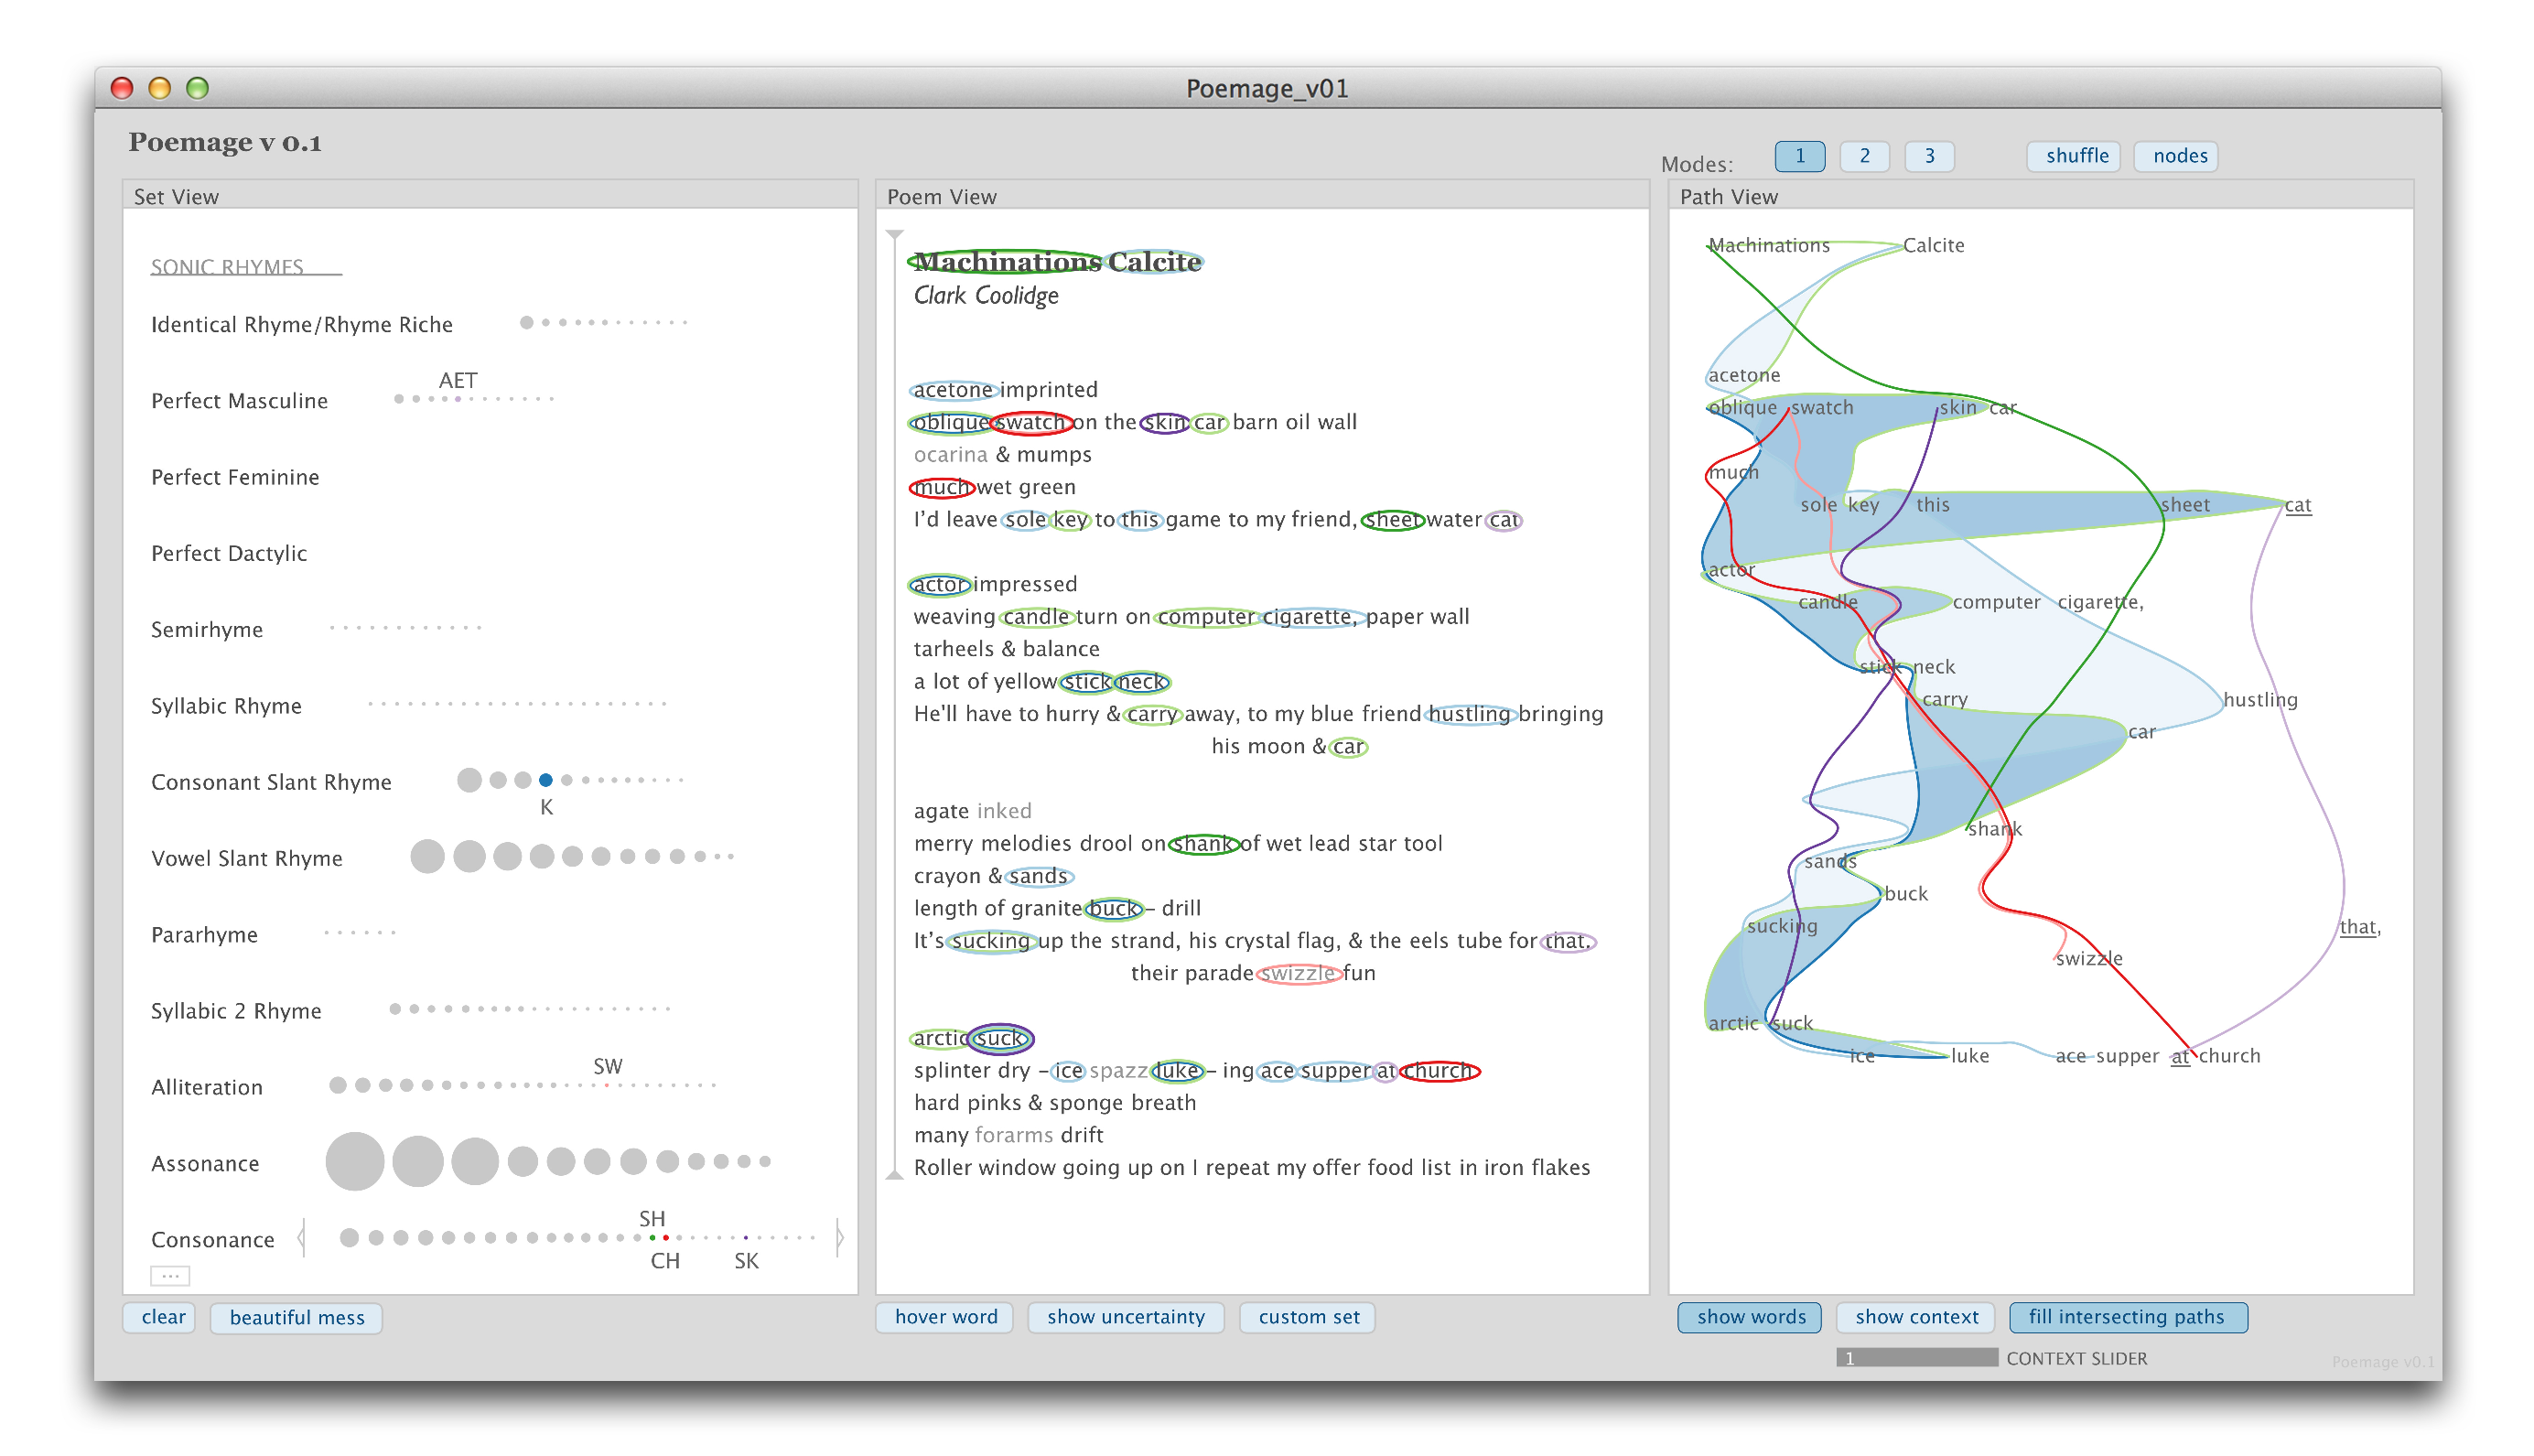
\includegraphics[scale=0.24]{../img/poemage.pdf}
	\caption{An example analysis in Poemage.}\label{screenshotPoemage}
\end{figure}

\subsection*{Ambiances}
This software is unique in the fact that the analysis is integrated in the process of writing. As described in the paper \cite{Meneses2015}, writers input the poem, receive a visualization and can control this visualization with body and hand gestures which in turn influence the poem. By such interconnection the authors aim to make Ambiances a part of the writing process and give it a chance to influence the final result. However, the actual software does not seem to be publicly available.


\section{Generation tools}\label{generation_tools}

Generation of text, especially artistic, is a very challenging task for a machine. As we observed the outputs of exiting tools, we found that the most common flaws include lack of creativity, unnatural and frequent change of the subject, and incoherence. Generation of song lyrics is basically a more specified
\MP{Nemyslíte specific?}
branch of text generation. Similarly, it can be distinguished into two main \added{types of} methods -- rule-based and machine learning.
\MP{similarly to what? Asi Similarly to rhyme detection.}

\subsection{Rule-based generating}
Rule-based \replaced[comment={Model značí něco natrénovaného pomocí machine learning, tedy ne rule-based.}]{tools}{models} are inherently very complex and the output is often limited to certain structure or topic. They usually require the user to input starting configuration, whether it is genre, topic, time period, amount and type of rhymes, phrases, etc. They tend to be less creative but better at rhyming and following the form and structure. To achieve that, they may use rhyming dictionaries (see Section \ref{rhyme_detection_tools}). Simpler ones just use a large set of pre-written templates, e.g. MasterPiece Generator.\footnote{\url{https://www.song-lyrics-generator.org.uk/}} In this thesis, we will focus on generation using artificial intelligence (AI).
\MP{Obecně se AI považuje za nadmnožinu machine learning (což je nadmnožina deep learning, což se velmi překrývá s artificial neural networks).
Do AI tradičně spadají i rule-based metody.
Buď vysvětlete čtenáři, že pod AI rozumíte jen moderní machine-learning-based AI,
 nebo změňte tuto větu a následující podsekci přejmenujte.
Chtělo by to ale ověřit, že všechny uvedené online generátory jsou opravdu machine-learning based.
Tipuji, že některé budou spíš pravidlové.
Pokud to o nich víte, uveďte je v této podsekci.
Samozřejmě mohou existovat metody hybridní využívající jak ručně psaná pravidla, tak strojové učení.
Jedním z příkladů je nakonec Váš detektor.
}

\subsection{Generating using AI}
The go-to approach for generating song lyrics is certainly AI in its many forms.
\MP{go-to mi jednak nepřijde vhodné pro odborný styl, jednak to vnímám v podstatě jako best,
což je sporné tvrzení -- pokud do AI nezahrnujeme rule-based, tak třeba nějaké roky vylepšované rule-based řešení může být nejlepší.
Pokud zahrnujeme, tak je otázka, zda vůbec existují nějaké plně automatické non-AI metody
a zda má ta věta vůbec nějakou výpovědní hodnotu.
}
It can be proved by the large number of AI lyrics generators created by enthusiasts, e.g. \textit{These Lyrics Do Not Exist}\footnote{\url{https://theselyricsdonotexist.com/}}, \textit{Freshbots Lyrics Generator}\footnote{\url{https://www.freshbots.org/lyrics-generator}}, \textit{Random Lyrics Generator}\footnote{\url{http://www.anticulture.net/RandomLyrics.php}}, \textit{DeepBeat -- Rap Lyrics Generating AI}\footnote{\url{https://deepbeat.org/}}, \textit{BoredHumans Generator}\footnote{\url{https://boredhumans.com/lyrics_generator.php}}, \textit{RapPad Lyrics Generator}\footnote{\url{https://www.rappad.co/songs-about/}}, and many more. We will further describe Deep-speare (mentioned earlier in Section \ref{ml}) and current state-of-art GPT-2 and GPT-3.
\MP{Jednak state-of-\textbf{the}-art.
Jednak by mělo být jasné, v kterém ohledu jsou state-of-the-art,
 tedy nejspíš v nějaké měřitelné evaluaci.
U benchmarků typu GLUE a SuperGLUE už jsou myslím i lepší modely,
 ale není to dávno, co bylo na prvních příčkách GPT, takže tam by to pojmenování šlo použít.
Zde nás ale spíš zajímá generování poezie a v tom nevím o žádném benchmarku a ustáleném způsobu evaluace.
Možná by šlo něco jako ``and GPT models, which are considered state of the art in text generation.''
}

\subsubsection*{Deep-speare}
Deep-speare (\cite{lau2018deep}) is a joint neural network architecture that generates only a specific type of poems with strict form and meter -- \gls{sonnet} \gls{quatrain}s. It consists of three models: language model generates one word at a time, pentameter model samples meter-conforming sentences, rhyme model enforces rhyme, and they are all trained together in multi-task learning setting. They present very good results -- generated poems are mostly indistinguishable from human-written ones, apart from expert evaluation, where they report lack of emotion and worse readability.

\subsubsection*{GPT-2}
Generative pre-trained Transformer version 2 (GPT-2) (\cite{radford2019gpt2}) is an unsupervised \gls{transformer_model} capable of various text-processing and generating tasks such as answering questions, translating, summarizing, writing coherent paragraphs, etc. It was created by AI-based research laboratory named OpenAI.

This model was trained on and evaluated against WebText, a dataset consisting of the text contents of 45 million links on sites like Google, Blogspot, GitHub, NYTimes, BBC, eBay, etc. It offers 4 models of different sizes increasing in the number of parameters: 124 million (small), 355 million (medium), 774 million (large), and 1.5 billion (XL) parameter models.

Although this model was only trained for the general task of predicting the next word, given all of the previous words within some text, it can be further fine-tuned for a more specific task to suit user's needs. However, even without fine-tuning, it can quickly adapt to the style of the input and continue in the same manner. One example of lyrics generated by GPT-2 is \textit{Keywords To Lyrics}\footnote{\url{https://lyrics.mathigatti.com/}}.
\MP{Jenže zrovna toto je fine-tunované na písničkách, viz https://github.com/mathigatti/pop-lyrics-dataset
Stačí tedy změnit pořadí těch posledních dvou vět.
Po tom ``continue in the same manner'' by ještě měl následovat odkaz na Vaše experimenty v Kapitole 6.}

\subsubsection*{GPT-3}
During writing of this thesis, an even larger model GPT-3 (\cite{brown2020gpt3}) with 175 billion parameters was officially introduced. It is considered the largest artificial neural network created to date.
\MP{Radši It was considered... in May 2020. Ono se to rychle mění.
Zaznamenal jsem třeba Google Switch Transformer 6krát větší než GPT-3, ale jsou i další:
https://towardsdatascience.com/top-5-gpt-3-successors-you-should-know-in-2021-42ffe94cbbf
}
It was trained on five different corpora: Common Crawl, WebText2, Books1, Books2 and Wikipedia. The architecture is the same as in GPT-2, only number of layers and other parameters increased. It is capable of writing articles indistinguishable from human-written ones,
\MP{Zde by se velmi hodila citace.}
even produce functional JavaScript code for natural-language formulated task.

Realizing the power of this tool, the authors did not want to make it available to broad public, fearing it might be misused with bad intentions. Instead they created a form to sign up for access, reviewed individual requests, granting access only to a small portion of them.



\paragraph{}Originally, this thesis intended to focus more on lyrics generation. However, as our research of works in this field shows, there is an abundance of tools for \added{that} purpose. Users can just choose a tool that fits their needs. Creating one tool that would be better or more versatile would either require more computing power or literary knowledge, and is above the scope of a master thesis. Therefore, we shifted our main focus to automatic rhyme detection and evaluation, which seems to be far less explored and more interesting topic.


